\chapter{\index{vettore}Vettori}
\minitoc
Un vettore è rappresentabile con un segmento orientato, ogni vettore individua un punto e viceversa. Un vettore è un ente geometrico, ovvero è indipendente dalla rappresentazione. Fissata una base, nel caso usuale una terna ortonormale di vettori, ogni vettore è rappresentato da una terna di coordinate cioè da un elemento di $\field{R}^3$. Un modo equivalente per rappresentare un vettore è tramite modulo, direzione e verso. Il modulo, o norma del vettore, è la lunghezza del segmento, la direzione è la retta passante per il segmento, il verso indica l'orientazione del vettore. Nei libri i vettori sono in grassetto\footnote{altre notazioni sono $\underline v$, $\vec{v}$}. $\ve{v}$ è un vettore, $|\ve{v}|$, $\norm{\ve v}$ o semplicemente $v$ è il modulo del vettore.

I vettori sono da intendersi applicati nell'origine. Si può anche trattare di vettori non applicati nell'origine, chiamandoli vettori applicati, ma si rivelano del tutto equivalenti ai vettori usuali, infatti spesso gli si pensa come elementi di classi di equivalenza i cui rappresentati sono i vettori applicati nell'origine.
\begin{figure}[htbp]
  \centering
  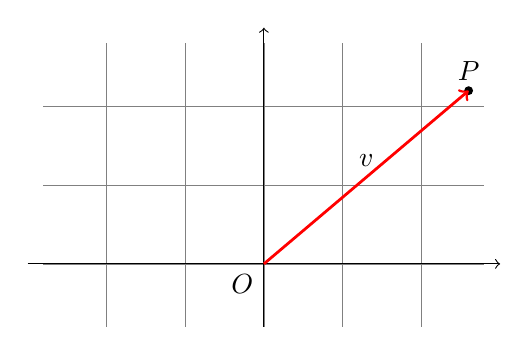
\begin{tikzpicture}[scale=2]
  \clip (-1.5,-0.4) rectangle (1.5,1.5);
  \draw[step=.5cm,gray,very thin] (-1.4,-1.4) grid (1.4,1.4);
  \draw[->] (-1.5,0) -- (1.5,0);
  \draw[->] (0,-1.5) -- (0,1.5);
  \fill (1.3,1.1) circle (0.8pt) node[above]{$P$};
  \draw[red,line width=1pt, ->] (0,0) node[below left, black] {$O$} -- (1.3,1.1) node[midway, above, black] {$\ve v$};    
\end{tikzpicture}

  \caption{Vettore $\ve v$ applicato nell'origine che individua il punto $P$.}
\end{figure}
\section{\index{versore}Versori e \index{coordinate}coordinate}
I versori sono vettori della base ortonormale di $\field{R}^3$ (lo spazio) considerato con il prodotto scalare canonico. In parole povere sono sono vettori di modulo unitario ortogonali a due a due. Solitamente si indicano con $\ver i$, $\ver j$ e $\ver k$ i versori applicati nell'origine, nella direzione degli assi cartesiani del sistema di riferimento. Le loro coordinate sono\footnote{quando si scrive che $\ve v=(a,b,c)$ l'uguaglianza significa che che fissata una base il vettore è rappresentato dalle sue coordinate $(a,b,c)$, ma vettori e coordinate non sono la stessa cosa, per esempio se si fa un cambiamento di base il vettore non cambia, ma le sue coordinate sì.}:
\[
  \ver \imath=\left(\begin{array}{c} 1\\0\\0\\ \end{array}\right)\qquad
  \ver \jmath=\left(\begin{array}{c} 0\\1\\0\\ \end{array}\right)\qquad
  \ver k=\left(\begin{array}{c} 0\\0\\1\\ \end{array}\right)
\]

Poiché i versori formano una base ogni vettore può essere espresso come una loro combinazione lineare, i coefficienti sono le coordinate\footnote{come già accennato i due simboli di uguaglianza hanno significati diversi, il primo è una vera uguaglianza, il secondo vuol dire che fissata una base, il vettore è rappresentato da quelle coordinate.}:
\[
  \ve v=v_x\ve i+v_y\ve j+v_z\ve k=\left(
  \begin{array}{c}
      v_x \\v_y\\v_z\\
    \end{array}\right)
\]
\section{Individuazione vettori}
\begin{figure}[htbp]
  \centering
  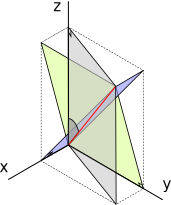
\includegraphics{immagini/fisica1/vettore_geometrico}
  % vettore_geometrico.pdf: 161x165 pixel, 72dpi, 5.68x5.82 cm, bb=0 0 161 165
  \caption{l'angolo evidenziato è l'angolo $\alpha$ tra il vettore e l'asse $z$. Quest'angolo appartiene al piano individuato dal vettore e dall'asse $z$ (in grigio).}
\end{figure}
I vettori si possono individuare in un sistema di riferimento per via geometria o per via analitica. Individuando un vettore per via geometrica si indica il modulo, e gli angoli che il vettore forma con gli assi cartesiani. Nello spazio:
\[
  \left\{
  \begin{array}{l}
    |\ve v| \\
    \alpha,\beta,\gamma
  \end{array}\right. \qquad \text{con}\qquad \cos^2 \alpha+\cos^2 \beta + \cos^2
  \gamma=1
\]
Notiamo che gli angoli $\alpha$, $\beta$ e $\gamma$ non sono indipendenti, possiamo ricavarne uno in funzione degli altri; quindi un vettore sarà descritto da tre informazioni, per esempio $|\ve v|$, $\alpha$, $\beta$.

Per via analitica invece bisogna indicare le componenti del vettore rispetto alla base $\{\ve i, \ve j, \ve k\}$: $\left(
  \begin{array}{l}
      v_x \\v_y\\v_z
    \end{array}\right)
$.
\subsection{Passaggio da individuazione geometrica a individuazione analitica}
\[
  \left\{
  \begin{array}{l}
    v_x=|\ve v|\cos\alpha \\
    v_y=|\ve v|\cos\beta  \\
    v_z=|\ve v|\cos\gamma
  \end{array}
  \right. \qquad \qquad \left\{
  \begin{array}{l}
    |\ve v|^2=v_x^2+v_y^2+v_z^2     \\
    \cos\alpha=\cfrac{v_x}{|\ve v|} \\
    \cos\beta=\cfrac{v_y}{|\ve v|}  \\
    \cos\gamma=\cfrac{v_z}{|\ve v|}
  \end{array}
  \right.
\]


\section{Operazioni tra i vettori}

\subsubsection{Vettore inverso}
Il vettore inverso ha stesso modulo del vettore, stessa direzione,
ma verso opposto.
\[
  -\ve v=-(v_x\ve i+v_y\ve j+v_z \ve k)=-v_x\ve i-v_y\ve
  j-v_z\ve k
\]
Naturalmente ogni vettore ha inverso e la loro somma è nulla e $-\ve 0=\ve 0$.

\subsubsection{Somma}
La somma di due vettori è il vettore che ha come componenti la somma delle componenti. Dal punto di vista grafico equivale a usare la regolare del parallelogramma:
\begin{multline*}
  \ve a+\ve b=(a_x\ve i+a_y\ve j+a_z \ve k)+(b_x\ve
  i+b_y\ve j+b_z\ve k)=\\
  =(a_x+b_x)\ve i+(a_y+b_y)\ve
  j+(a_z+b_z)\ve k
\end{multline*}

\begin{figure}[htbp]
  \centering
  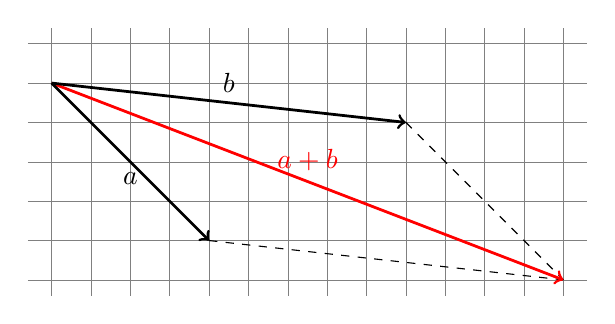
\begin{tikzpicture}[scale=1]
  \draw[step=.5cm,gray,very thin] (-2.3,-1.7) grid (4.8,1.7);
  \coordinate (A) at (-2,1);
  \coordinate (B) at (-0,-1);
  \coordinate (C) at (2.5,0.5);
  \coordinate (D) at (+2.5+2,-1+0.5-1);
  \draw[dashed] (B) -- (D);
  \draw[dashed] (C) -- (D);
  \draw[line width=1pt, red, ->] (A) -- (D) node[midway, above] {$\ve a + \ve b$};
  \draw[line width=1pt, ->] (A) -- (B) node[midway, below] {$\ve a$};
  \draw[line width=1pt, ->] (A) -- (C) node[midway, above] {$\ve b$};
\end{tikzpicture}

  \caption{Regola del parallelogramma.}
\end{figure}

\subsubsection{Differenza} La differenza di due
vettori è la somma del primo con l'inverso del secondo. Graficamente $\ve a-\ve b$ è il vettore che congiunge $\ve b$ ad $\ve a$.
\subsubsection{Prodotto per uno scalare}
Per via geometrica il prodotto scalare di un vettore per uno scalare corrisponde al vettore con stessa direzione, con modulo moltiplicato per il valore assoluto dello scalare e verso invertito se lo scalare è negativo.
\[\forall h \in \field{R}\qquad h\ve a=h(a_x\ve i+a_y\ve j+a_z\ve k)=ha_x\ve i+ha_y\ve j+ha_z\ve k\]
\subsubsection{\index{prodotto!scalare}Prodotto scalare}
Il prodotto scalare usato in fisica è il prodotto scalare canonico della geometria in $\field{R}^3$ rispetto alla base canonica $\{\ve i,\ve j,\ve k\}$:
\[\left(\ve{x},\ve{y}\right)=\ve{x}^T\cdot\ve{y}=(x_1y_1+x_2y_2+x_3y_3)\]
\[p_s=|\ve a||\ve b| \cos \alpha\]
con $\alpha$ l'angolo compreso tra i due vettori. Da qui si deduce che $\ve i \cdot \ve i=1$, $\ve i
  \cdot \ve j=0$, ecc., che due vettori ortogonali hanno prodotto scalare nullo e che due vettori hanno prodotto scalare massimo quando sono paralleli.
\[p_s=\ve a \cdot \ve b=(a_x\ve i+a_y\ve j+a_z\ve k)\cdot(b_x\ve
  i+b_y\ve j+b_z\ve k)=a_xb_x+a_yb_y+a_zb_z\]
\subsubsection{\index{prodotto!vettoriale}Prodotto Vettoriale}
Matematicamente il prodotto vettoriale non è facile da definire. Esso restituisce un vettore che ha direzione ortogonale al piano individuato dai due vettori, verso ricavabile dalla regola della mano destra, e modulo:
\[|\ve p_v|=ab\sin \alpha\] con $\alpha$ angolo tra i due vettori\footnote{è molto semplice ricordarsi la formula del prodotto vettoriale, basta ciclare sulle variabili. Per esempio la componente $x$ del prodotto vettoriale è $a_yb_z-a_zb_y$ in cui l'ordine è $x$ (la componente) e poi $y$, $z$, seguito dalla sottrazione al contrario (è antisimmetrico)}.


\begin{align*}
  \ve p_v & =\ve a \wedge \ve b=\ve a \times \ve b=(a_x\ve i+a_y\ve j+a_z\ve k)\wedge(b_x\ve
  i+b_y\ve j+b_z\ve k)                                                                       \\
          & =(a_yb_z-a_zb_y)\ve i+(a_zb_x-a_xb_z)\ve j+(a_xb_y-a_yb_x)\ve k
\end{align*}

Il prodotto vettoriale può essere calcolato come determinante di una matrice $3\times 3$:
\[\ve p_v=
  \left| \begin{array}{ccc} \ve i & \ve j & \ve k \\
             a_x         & a_y   & a_z   \\
             b_x         & b_y   & b_z
  \end{array} \right|\]

Il prodotto vettoriale è antisimmetrico cioè $\ve a \wedge \ve
  b=-\left(\ve b \wedge \ve a\right)$. Il modulo del prodotto
vettoriale è l'area del parallelogramma avente come lati i due
vettori.

Il prodotto vettoriale è dipendente dalla scelta del sistema di riferimento.
In Figura~\ref{fig:sistema_destrogiro} sono illustrati il sistemata destrogiro e sinistrogiro, che seguono la regola della mano destra o della mano sinistra.
In particolare il verso del prodotto vettoriale segue la regola della mano destra se il sistema di riferimento è destrogiro, altrimenti il verso risulta opposto. Per questo il prodotto vettoriale è chiamato pseudovettore. In natura le grandezze osservabili non devono dipendere dalla scelta dell'orientazione (chiralità) degli assi cartesiani. Per convenzione si sceglie un sistema di riferimento destrogiro.
\begin{figure}[htbp]
  \centering
  \subfigure[destrogiro]{\begin{tikzpicture}[scale=2]
  \draw[->] (0,0) -- (1.5,0) node[at end, above] {$y$};
  \draw[->] (0,0) -- (0,1.5) node[at end, above] {$z$};
  \draw[->] (0,0) -- (-1/2., -1.73/2.) node[at end, above] {$x$};
\end{tikzpicture}
}
  \subfigure[sinistrogiro]{\input{immagini/fisica1/sistema_sinistrogiro}}
  \caption{Coordinate destrogire e sinistrogire}
  \label{fig:sistema_destrogiro}
\end{figure}

\subsubsection{\index{prodotto!misto}Prodotto Misto}
Il prodotto misto è definito come:
\[p_m=\ve c\cdot\left(\ve a \wedge \ve b\right)\]
Esso è uguale all'area del parallelepipedo avente come spigoli i
vettori \mbox{$\ve a$, $\ve b$, $\ve c$.}

\subsubsection{\index{derivata!di un vettore}Derivata di un vettore}
La derivata di un vettore è la derivata delle coordinate per i rispettivi versori, (i versori sono costanti). Per esempio la derivata della velocità rispetto al tempo è:
\[\frac{\ud\ve v}{\ud t}=\frac{\ud v_x}{\ud t}\ve i+\frac{\ud v_y}{\ud t}\ve j+\frac{\ud v_z}{\ud t}\ve k\]

\subsubsection{\index{gradiente}Gradiente}
\label{gradiente}
Il gradiente di uno scalare è definito come:
\[
  \grad V(x,y,z)=\ve\nabla V(x,y,z)=\frac{\partial V}{\partial x}\ver i + \frac{\partial V}{\partial y}\ver j +\frac{\partial V}{\partial z}\ver k +
\]
dove $\ve\nabla$ è un operatore definito come:
\[
  \ve\nabla=\left(\frac{\partial}{\partial x},\frac{\partial}{\partial y},\frac{\partial }{\partial z}\right)
\]
con questo operatore abbiamo il divertimento di scrivere le nostre formule per esempio in questo modo:

\[
  \ve F=-\ve\nabla U
\]
invece di:
\[
  \ve F=-\left(\frac{\partial U}{\partial
    x}\ve i+\frac{\partial U}{\partial y}\ve j+\frac{\partial
    U}{\partial z}\ve k\right)
\]